\documentclass[12pt]{article}
\usepackage[draft]{moodle}
\usepackage{fontspec}
\usepackage[brazilian]{babel}
%\usepackage[utf8]{inputenc}
%\usepackage[T1]{fontenc}
\usepackage{graphicx}
\ifwindows\imagemagickcommand{magick convert}
\else\imagemagickcommand{convert}
\fi

\begin{document}
	\begin{quiz}{MudancasDeFaseObjetivaFacil}
		\begin{multi}[points=1]{MDF01OF-B}
			\textbf{(IBMEC SP Insper/2017)} Passamos, neste ano de 2016, por um inverno bastante rigoroso nas regiões Sul e Sudeste do país. Nas localidades habitualmente frias da Terra, os imóveis necessitam ter um sistema de aquecimento para que as pessoas possam viver sentindo-se bem. No Brasil, são poucas as construções que já apresentam infraestrutura de aquecimento instalada. Em geral, os aquecedores podem ser elétricos, a gás ou a óleo, portáteis ou fixos, e serem do tipo a resistência, termoventilador, radiador etc.\\			
			Descartando a questão do custo de instalação e pensando apenas na maneira mais eficiente e uniforme de distribuir o ar quente pelo ambiente, o sistema mais indicado é o			
			\item termoventilador dotado de uma resistência aquecedora, que melhora a eficiência e a velocidade de distribuição do ar quente.
			\item* piso radiante a água ou a cabo, em que uma serpentina na qual circula água aquecida ou um cabo aquecido por corrente elétrica são ambos colocados sob o piso.
			\item ar condicionado frio-quente, modelo Split, localizado no alto de uma parede.
			\item aquecedor a óleo, dotado de uma resistência interna que aquece o óleo que circula por uma serpentina junto a uma parede.
			\item radiador, instalado no chão, junto a uma parede para não interferir na circulação das pessoas.
		\end{multi}
	
		\begin{multi}[points=1]{MDF02OF-D}
			\textbf{(UECE/2016)} A humanidade acaba de chegar ao meio de um caminho considerado sem volta rumo a mudanças climáticas de grande impacto. Um estudo divulgado pelo serviço britânico de meteorologia mostrou que a temperatura média da Terra teve um aumento de 1,02 ºC no período correspondente ao início da Revolução Industrial até os dias atuais. É a primeira vez que se registra um aumento dessa magnitude e se rompe o patamar de 1 ºC, um flagrante desequilíbrio no planeta. A fonte predominante e a forma de transmissão dessa energia térmica que chega à Terra é, respectivamente,					
			\item o sol e a convecção.
			\item o efeito estufa e a irradiação.
			\item o efeito estufa e a circulação atmosférica.
			\item* o sol e a irradiação.
		\end{multi}
		\begin{multi}[points=1]{MDF03OF-A}
			\textbf{(IFSP/2016)} Observando um refrigerador, a geladeira comum de sua casa, um aluno escreveu as seguintes afirmações:\\			
			I.	A energia na forma de calor que sai dos alimentos chega ao congelador pelo processo de convecção na maior proporção e muito pouco por radiação.\\
			II.	O congelador está situado na parte superior para receber o ar aquecido pelo calor dos alimentos.\\
			III. As camadas que formam as paredes da geladeira são intercaladas por material isolante para evitar a entrada de calor por condução.\\
			IV.	Os espaços internos são divididos por grades vazadas que facilitam o movimento por convecção das massas do ar quente e frio.\\			
			As afirmativas corretas são:							
			\item* I, II, III e IV.
			\item I, II e III, apenas.
			\item II e IV, apenas.
			\item II, III e IV, apenas.
			\item III e IV, apenas.
		\end{multi}
		\begin{multi}[points=1]{MDF04OF-C}
			\textbf{(UNEMAT MT/2016)} No início do processo de cozimento de alimentos, observa-se o deslocamento da água no interior da panela, que ocorre devido ao empuxo, em que o líquido se desloca conforme a sua densidade. Desta forma, a água quente sobe e a água fria desce, efetuando a troca de calor no líquido.\\			
			Assinale a alternativa que se refere a este processo de troca de calor.										
			\item Radiação.
			\item Contato.
			\item* Convecção.
			\item Atrito.
			\item Deslocamento.
		\end{multi}
		\begin{multi}[points=1]{MDF05OF-C}
			\textbf{(UFU MG/2016)} Em Los Angeles, Estados Unidos, fumaça e outros poluentes atmosféricos constituem o smog, que fica aprisionado sobre a cidade, devido a um fenômeno chamado “Inversão de temperatura”. Isso ocorre quando o ar frio e de baixa altitude, vindo do oceano, é retido sob o ar quente que se move por cima das montanhas, vindo do deserto de Mojave. O fenômeno é representado no esquema a seguir:
			\begin{center}
				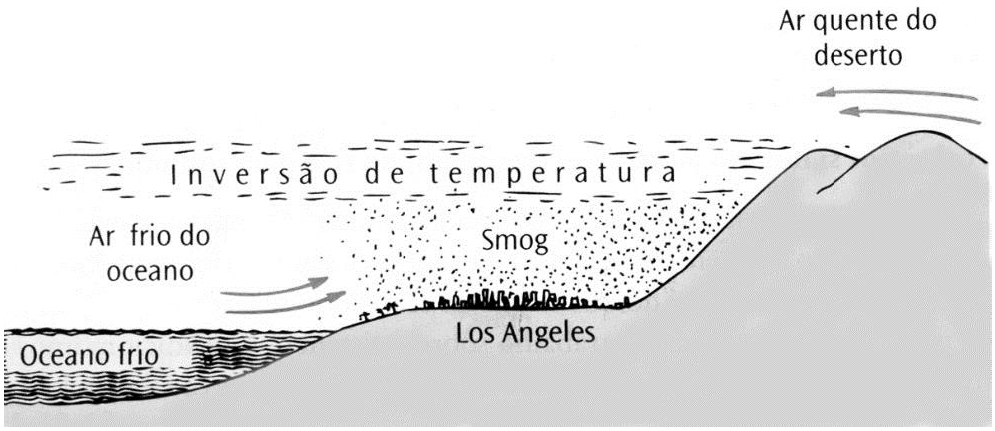
\includegraphics[width=0.7\linewidth]{img3}\\HEWITT, P. G. Física Conceitual. 11ª ed. Porto Alegre: Bookman, 2011.			
			\end{center}
			A principal propriedade física do smog, que dificulta sua dispersão, é			
			\item sua umidade relativa.
			\item seu calor específico.
			\item* sua densidade.
			\item seu coeficiente de dilatação volumétrico.	
		\end{multi}	
		\begin{multi}[points=1]{MDF06OF-A}
			\textbf{(UEA AM/2016)} Devido ao forte calor em Manaus, é comum a instalação de aparelhos de ar condicionado, principalmente em locais públicos fechados. O ar resfriado pelo aparelho de ar condicionado troca calor com o ambiente interno principalmente por	
			\item* convecção e esse processo necessita de um meio material para se realizar.
			\item convecção e esse processo ocorre nos meios materiais e no vácuo.
			\item irradiação e esse processo não ocorre nos meios materiais e no vácuo.
			\item condução e esse processo depende da umidade do ar, que é um meio material.	
			\item condução e esse processo não ocorre nos meios materiais e no vácuo.
		\end{multi}
		\begin{multi}[points=1]{MDF07OF-D}
			\textbf{(ENEM/2016)} Para a instalação de um aparelho de ar-condicionado, é sugerido que ele seja colocado na parte superior da parede do cômodo, pois a maioria dos fluidos (líquidos e gases), quando aquecidos, sofrem expansão, tendo sua densidade diminuída e sofrendo um deslocamento ascendente. Por sua vez, quando são resfriados, tornam-se mais densos e sofrem um deslocamento descendente.\\			
			A sugestão apresentada no texto minimiza o consumo de energia, porque				
			\item diminui a umidade do ar dentro do cômodo.
			\item aumenta a taxa de condução térmica para fora do cômodo.
			\item torna mais fácil o escoamento da água para fora do cômodo.
			\item* facilita a circulação das correntes de ar frio e quente dentro do cômodo.
			\item diminui a taxa de emissão de calor por parte do aparelho para dentro do cômodo.
		\end{multi}
		\begin{multi}[points=1]{MDF08OF-C}
			\textbf{(Unievangélica GO/2015)} A lei de Stefan-Boltzmann conecta a potência irradiada por um corpo negro para todas as frequências com relação à área superficial emissora e sua temperatura absoluta.\\			
			Nessa lei, a temperatura tem uma dependência						
			\item linear
			\item quadrática
			\item* quádrupla
			\item cúbica
		\end{multi}
		\begin{multi}[points=1]{MDF09OF-C}
			\textbf{(UFT TO/2014)} Uma sala de estúdio é mantida à temperatura de 20 ºC e se encontra separada de uma sala vizinha, à temperatura ambiente de 30 ºC, por uma janela retangular de vidro, de 8,0 mm de espessura, 1,0 m de altura por 1,5 m de largura. Sabendo que a condutividade térmica do vidro é 0,80 W/m.K, o total de calorias transmitidas pela janela, após 4,2 minutos é de, aproximadamente:								
			\item 1,50 kcal.
			\item 37,8 kcal.
			\item 60,0 kcal.
			\item* 90,0 kcal.
			\item 126 kcal. 
		\end{multi}
		\begin{multi}[points=1]{MDF09OF-C}
			\textbf{(ENEM/2013)} Em um experimento, foram utilizadas duas garrafas PET, uma pintada de branco e a outra de preto, acopladas cada uma a um termômetro. No ponto médio da distância entre as garrafas, foi mantida acesa, durante alguns minutos, uma lâmpada incandescente. Em seguida, a lâmpada foi desligada. Durante o experimento, foram monitoradas as temperaturas das garrafas: a) enquanto a lâmpada permaneceu acesa e b) após a lâmpada ser desligada e atingirem equilíbrio térmico com o ambiente.
			\begin{center}
				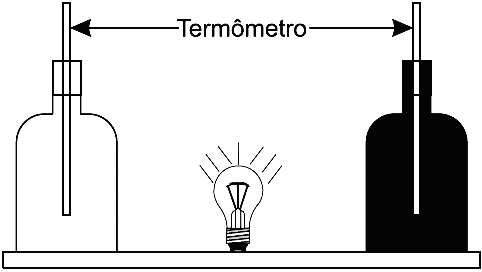
\includegraphics[width=0.7\linewidth]{img10}		
			\end{center}		
			A taxa de variação da temperatura da garrafa preta, em comparação à da branca, durante todo experimento, foi											
			\item igual no aquecimento e igual no resfriamento.
			\item maior no aquecimento e igual no resfriamento.
			\item menor no aquecimento e igual no resfriamento.
			\item maior no aquecimento e menor no resfriamento.
			\item* maior no aquecimento e maior no resfriamento.
		\end{multi}										
	\end{quiz}
\end{document}